\chapter{MELON Implementation}\label{chapter:implementation}

This chapter describes a prototype implementation of MELON we developed in order to validate our design and obtain empirical performance data.

\section{Architecture}

\begin{figure}
\centering
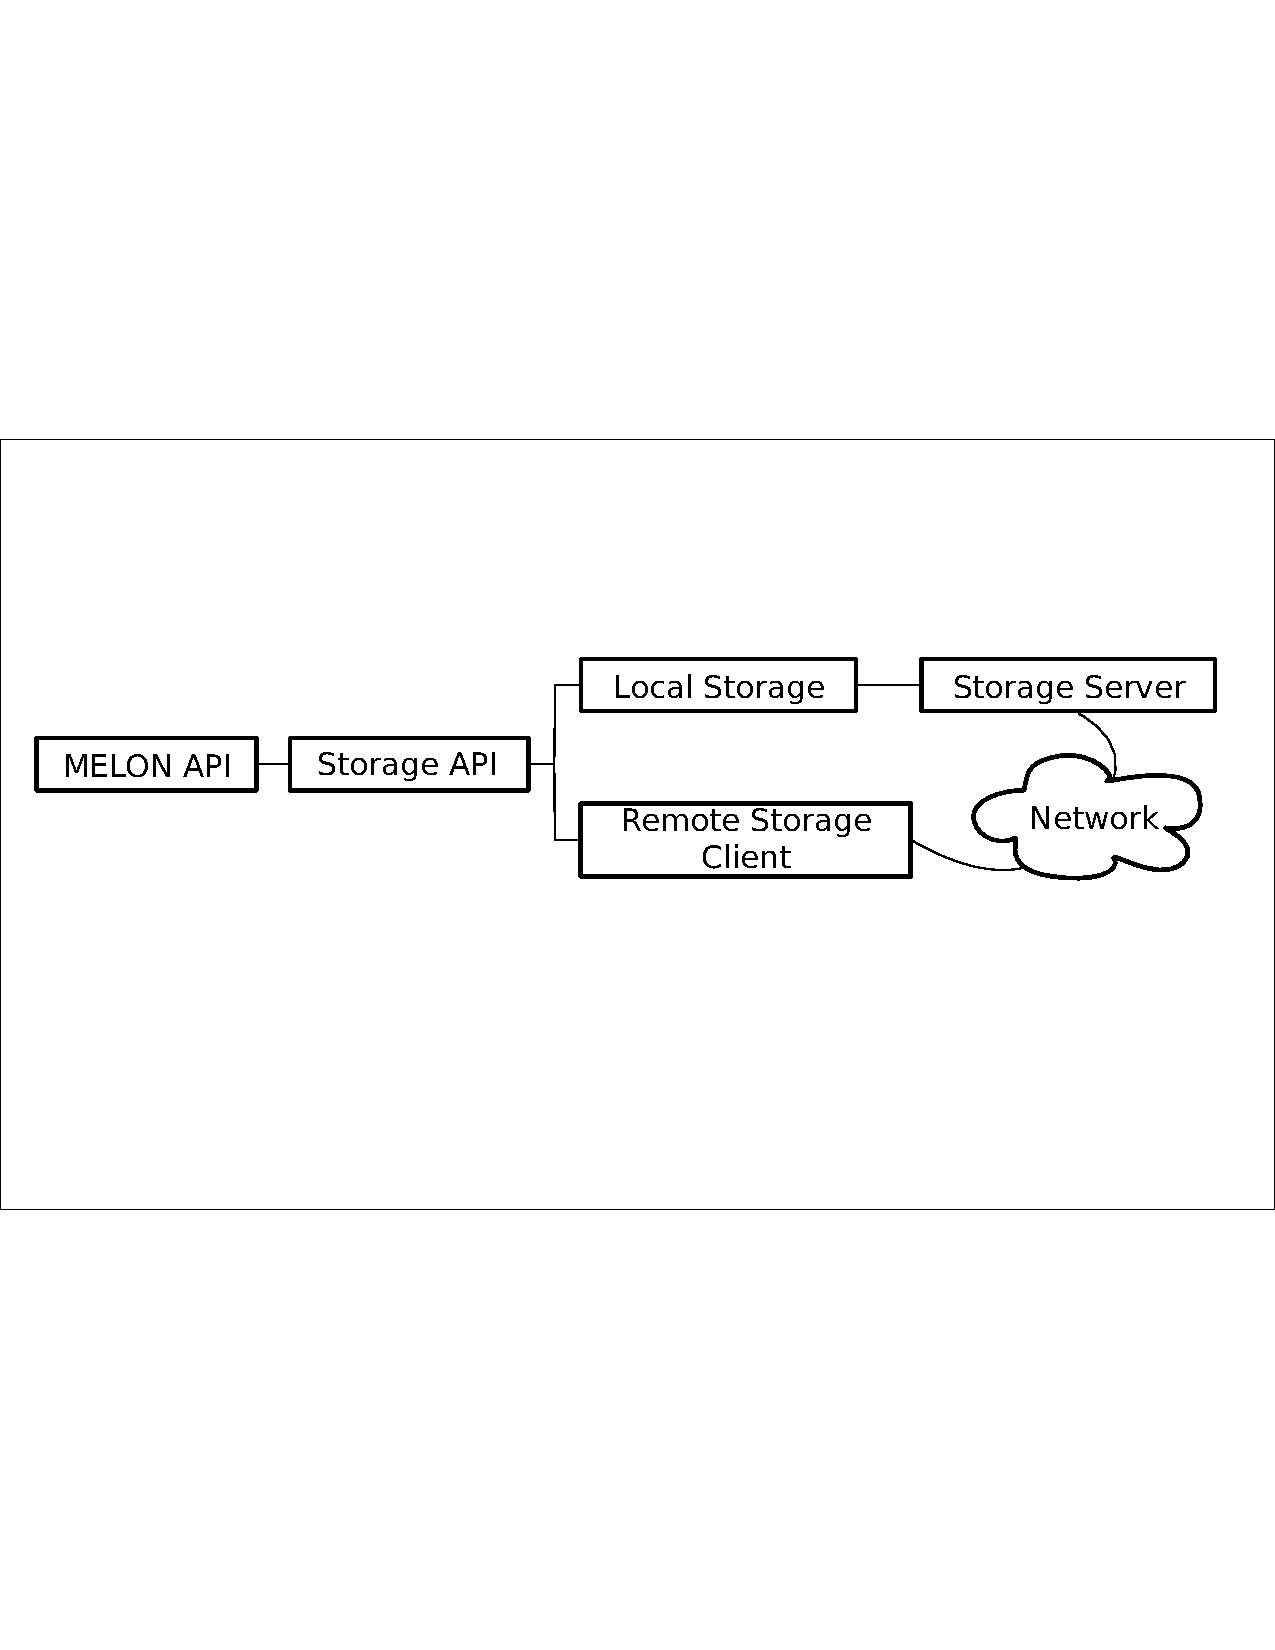
\includegraphics[scale = .70, clip, trim = 10px 280px 10px 250px]{figures/paradigm_arch.pdf}
\caption{Paradigm Architecture}
\label{fig:architecture}
\end{figure}

The architecture of our MELON implementation illustrated in Figure \ref{fig:architecture} is divided into five parts. The MELON API is the only interface exposed to the application and provides the six operations described above. The MELON API interacts with the distributed message storage through the storage API, which provides the same interface for both local and remote storage. The storage server proves a network interface to a local storage space and accepts connections made through the remote storage stub.

\section{MELON API}

The MELON API as provided to the application is very simple. It only provides the six MELON operations, plus the ability to manually specify remote hosts. The API implementation does very little except interact with either local or remote storage. Both local and remote storage offer the same API, so they can be accessed uniformly.

The prototype library tracks the local storage, remote servers, and read messages. \textbf{write} and \textbf{store} operate on the local storage only. \textbf{read} and \textbf{take} make no distinction between local and remote storage but simply iterate through the list of stores and invoke operations on them until the operation is satisfied. Each operation accesses the stores in a random order to spread the load and also provide a variety of sources.

\section{Storage API}

The storage API is an interface between the MELON API and either local or remote storage. In practice, however, the MELON API calls methods on the local storage directly. The API offers exactly the same six operations as MELON.

Remote storage is accessed through the remote storage client which implements the same API as local storage, except without \textbf{write}/\textbf{store} since those are only performed locally. Each remote host is represented with its own remote storage client. Internally, the remote storage clients manage connections with the remote storage servers.

\section{Local Message Store}

While applications view the message store as a single entity, it is actually the federation of local message stores hosted by each node running MELON. Each message in the network is by default stored on exactly one node, which is the node on which the application is running which performed the \textbf{store} or \textbf{write} operation. In other words, storing a message is a local operation. This allows MELON to provide atomicity for message removal with \textbf{take} and to ensure per-host FIFO ordering when returning matched messages.

Local storage is implemented simply as two dynamic arrays, one for \textbf{write}/\textbf{read} messages and the other for \textbf{store}/\textbf{take} messages. For atomic updates, the \textbf{write}/\textbf{read} array uses a readers/writer lock to allow multiple \textbf{read} operations to access the array in parallel, but locks the array for \textbf{write} operations. The \textbf{store}/\textbf{take} array does not permit concurrent operations, since both \textbf{store} and \textbf{take} modify the store. The two arrays may be accessed and modified independently.

Implementation of \textbf{store}/\textbf{take} is simple: exclusive access is obtained for the appropriate array and the message is appended  to the end.

For \textbf{take}, the lock is obtained for the \textbf{store}/\textbf{take} array and the message store starts at the oldest message and linearly scans until a matching message is found. When a matching message is found, the message is removed from the array and the elements shift appropriately to fill the gap.

When performing a \textbf{read}, a readers lock for the \textbf{write}/\textbf{read} array is obtained. The message store starts at the oldest message and linearly searches the array for a matching message. If a message is matched, it must also be checked to not exist in the provided read message set (see Section \ref{sec:readmessages} below). If it is in the read message set, the search continues. Otherwise, the matching unread message is returned.

In the architecture described here, the local message store is unaware of the location of the requesting or storing client, although it is assumed \textbf{store}/\textbf{write} operations are local. The storage server provides an API for remote applications to connect to and query the local storage.

\section{Storage Server}

Each local storage is accompanied by a storage server which allows remote hosts to connect and query the local storage. The storage server handles incoming connections, converts queries into calls to the local storage, and converts messages from local storage into responses back to the remote hosts. Each storage server can handle multiple concurrent requests.

\section{Networking}

Network communication is handled using ZeroMQ\cite{hintjens2013zeromq}, a high performance, high level networking library. For the prototype, the network communication was intentionally kept simple. For example, a \textbf{read} request queries remote hosts in a random order and stops when a matching result is returned. For bulk operations, the prototype implementation also queries remote hosts in random order, but continues fetching results until all hosts have either returned a response or a timeout is reached.

While it is possible to improve upon this approach using multicast, it would greatly complicate the implementation by requiring the client to handle multiple asynchronous responses, choose between them, request the actual matching message, and then handle failure scenarios if the matching message cannot be returned. Our approach was to trade off potential performance gains for simplicity.

\section{Read Message Tracking}\label{sec:readmessages}

When a messages is stored, it is given a unique identifier [\textit{P}, \textit{M}], where \textit{P} is a globally unique integer identifier for the storing process, and \textit{M} is an integer identifier for the stored message. Each process maintains an integer ID which is incremented for each store. Messages stored from the same process with sequential \textbf{store} or \textbf{write} operations will have consecutive \textit{M} values and share the same \textit{P} value.

In order to prevent \textbf{read} from returning a message more than once in the same process, each process maintains a sparse bit set for each process from which a message has been read. The identifier [\textit{P}, \textit{M}] is condensed into a single unique integer \textit{Q} using the ``elegant pairing function''\cite{szudzikelegant} shown in Equation \ref{eq:elegantpairing}. Since the values of \textit{Q} will be consecutive integers for all consecutive values of $M < P$, it is helpful to set \textit{P} to be higher than the number of expected messages. The value \textit{Q} is then stored in a sparse bit set with a hash table using integer keys and bit field values.

 \begin{equation}
   f(M,P) = \left\{
     \begin{array}{lr}
       M^{2} + M + P & : M \geq P \\
       P^{2} + M & : M < P
     \end{array}
   \right.
   \label{eq:elegantpairing}
\end{equation}

The index \textit{i} in the sparse bit set indicates the range stored in the bit set. If \textit{w} is the number of bits for each bit set, then each bit field can store up to \textit{w} values of \textit{n}, where $w \times i \leq n < w \times (i + 1)$. A message with ID \textit{n} will be stored in index $n/w$ by setting the bit at $n \bmod w$ in the bit field to \texttt{1}.

If the index value is of size \textit{l} bits and the bit field contains \textit{w} bits, then the cost for storing a single value is $l + w$. For storing a set of consecutive values of length \textit{m}, the cost is $\lfloor \frac{m \times l}{w} \rfloor + m$ bits. In other words, the total cost is one bit per message, plus the cost of one index per \textit{w} messages.

\begin{table}
\centering
\caption{Sparse bit set example}
\begin{tabular}{|c|c|} \hline
Index & Bit Field \\ \hline
0 & 01100001 \\ \hline
4 & 00010000 \\ \hline
15 & 10100100 \\ \hline
\end{tabular}
\label{fig:bitset}
\end{table}

Consecutive messages (from any starting value) are the best-case scenario for sparse bit sets. In the worst case, the message IDs differ by at least \textit{w}, causing each message to incur a $l + w$ cost for storage and a total cost of $m \times (l + w)$ bits.

Determining if a message [\textit{P}, \textit{M}] is in the set is accomplished by first computing \textit{Q}. If there is no key at index $Q/w$, the message has not been read. Otherwise, retrieve the bit field \textit{b} at index $M / w$. If $b \wedge 2^{M \bmod w} \neq 0$ then the message has been read, otherwise the message is unread.

\section{Message Replication}\label{sec:replication}

Distributing copies of messages to multiple hosts can increase message availability when a host is temporarily unavailable, under heavy load, or even in the face of network partitioning. Additionally, it can improve performance if messages can be fetched from a nearer host or from multiple hosts in parallel. While not a requirement of the MELON paradigm, message replication may be implemented as an additional feature of MELON without adding any new operations although it does add complexity.

Take-only messages are generally not eligible for replication since their removal must be atomic. Coordinating removals for all replicated copies is not only impractical, it is impossible if a node containing a replicated message leaves the network. Read-only messages, however, are expected to be read many times and cannot be explicitly removed, making them a candidate for replication.

FIFO order (per host) must be maintained no matter which host may actually return the messages. When each host manages its own stored messages, ordering is easily accomplished. When messages are distributed and multiple copies of the same message are available from different hosts the problem is more challenging. However, each host is still aware of the order in which the messages should be returned.

Instead of sending a request for matching messages, a process requests a list of message IDs which would have fulfilled the request, in order. Each host responds with a list of matching message IDs, but only for messages output by that host. The requesting process can then request messages by ID rather than message templates. Any host may return the actual messages, either the original message or replicas. Since the requesting process will be aware of the correct ordering, it can ensure the FIFO ordering is maintained when returning messages to the application.

This approach still requires the original host to be available when the first request is sent, and it is limited to fetching messages which have already been output at the time of the request. As such, it is best fitted to bulk retrieval (\textbf{bulk\_read}) of messages.

One other type of message may be replicated. Take-only messages which are addressed to a specific receiver may also be safely replicated since they may only be removed by that receiver. The receiver can track which directed messages it has already taken and simply discard duplicates. Replicating messages which will only be needed once seems wasteful, though, except in the case where delivery of private messages is critical.

In any scenario, replicated messages would need to be kept in a separate storage from regularly output messages. Replicated messages would only be returned to requests by message ID or for directed take-only messages. A background process would be needed to replicate the messages out to different hosts. A mechanism would also be needed to determine when to replicate the messages, and when to garbage collect replicas. Overall, message replication requires a considerable amount of added complexity and overhead to MELON.

\section{Garbage Collection}

The MELON model explicitly acknowledges memory and storage are especially limited on mobile devices. For simplicity, in this section we consider this to be an absolute limit on the number of messages to be stored at any time. This is inexact in relation to the actually memory used since messages may vary in size.

Since MELON persists messages and read-only messages cannot be removed by applications, it would not be difficult for an application to exhaust available space on a device. This is an issue for any paradigm which persists its messages but most proposals do not address it. When there is no more space to store a message, a communication paradigm implementation may crash, raise an exception, simply drop the message, or perform garbage collection to remove existing messages and free space for new ones.

To offset its otherwise permanent storage of read-only messages, MELON implementations should have a mechanism to remove old messages. MELON's requirements for garbage collection straddle memory management garbage collection and cache eviction. In memory management, any references to a value in memory will require it to be kept, but MELON messages do not have direct references and we cannot know which messages may be needed in the future. This is similar to maintaining a cache, in which the same limitation of knowledge applies. Unlike a cache, there are generally no other copies of the message available to fall back upon. Once evicted from the MELON store, the message is lost.

First-in first-out (FIFO) and least-recently used (LRU) are basic strategies for choosing which messages to replace in storage. For MANET applications, there is often a few messages which are expected to be available for extended periods of time - for example, messages containing identity of nodes or other static data. This suggests simply discarding the oldest messages might not be the best approach. When evicting by LRU, it is necessary to track the last access time for each message. When deciding which messages to remove, the LRU policy drops the messages with the oldest access time. This is probably a good fit for MELON, but there are also more sophisticated variants on LRU which may be useful. Determining what replacement strategy is best for MELON is a topic for future work.

Besides determining which messages should be removed from storage, it is also necessary to have a policy for when to perform garbage collection. Unlike memory garbage collection, MELON garbage collection is not expected to have a significant impact on performance. MELON garbage collection does require locking the store to actually remove the messages, but the determination of which messages to remove may be performed without locking since it does not need to be exact. One approach is to only perform garbage collection when the message limit is actually reached, then to remove either a single message or a percentage of messages. Removing more messages reduces frequency of garbage collection, but increases the time spent removing messages each time.

Since MELON messages need to be stored in FIFO order, garbage collection does require some form of compacting to ensure new messages may be added at the end of the queue.

Fitting the best garbage collection strategy to MELON remains as future work.